\documentclass[11pt]{article}
\usepackage[margin=1in]{geometry}
\usepackage[T1]{fontenc}
\usepackage{booktabs,graphicx,hyperref,amsmath,array}
\usepackage[numbers]{natbib}
\title{Mentioned Is Not Binding: A Rules-plus-Small-Model Clause Ledger\\ and a Pre-registered Audit of Regex Extraction on US Federal Solicitations}
\author{Akteruzzaman Raihan Sikder\\ VETR Proposal, Acu-Elligent LLC\\ \small\texttt{araihansikder@gmail.com}}
\date{October 2026. Model: \url{https://huggingface.co/raihan-js/fedproc-ledger-v1}. Data: \url{https://huggingface.co/datasets/raihan-js/fedproc-ledger-bench}.}
\begin{document}
\maketitle

\begin{abstract}
Compliance tools for US federal contracting commonly build a ``clause ledger'' by finding FAR and DFARS clause numbers in a solicitation with regular expressions. We ask how well that status quo answers the question a contracting team actually has: which of the clauses \emph{bind} the contract? Without any annotator, we find that 13.8\% of the entries such regexes produce over 14{,}540 extracted solicitation documents (58{,}294 of 423{,}328) are clauses whose every mention is a checklist item with an empty box, and 20--31\% in checklist-heavy documents. We then build a rules layer (checkbox states, the unconditional paragraph (a) of FAR 52.212-5, inherited sub-item states, SF~1449 block 27, bare clause lists, exclusion vetoes) and a 0.46\,MB mention-role classifier, and evaluate against the status quo in seven pre-registered rounds on documents not used in any earlier round, including a temporal hold-out of solicitations posted after the last acquisition day. Labels come from a coding agent and two OpenAI models, not human experts. The first two rounds, with a labelling protocol that had a defect, did not show an advantage and one pre-registered hypothesis failed; after the rules were extended on development documents, four consecutive fresh rounds show higher binding-set F1 than the status quo (+0.14, +0.10, +0.11, +0.08; 95\% intervals above zero), specificity of 70--79\% against 8--19\%, and recall at or above the status quo's in three of four rounds. We report negative results (weakly labelled retraining, a number-level stacker, the failed rounds, a review queue that never met its target), an annotator-agreement ceiling (pairwise annotator agreement 75--82\%), and the main remaining error family. We release the model weights (pickle-free numpy archive with a numpy-only inference script), the per-mention table, all gold labels and round reports publicly.
\end{abstract}

\section{Introduction}
A US federal solicitation names its clauses in many ways: incorporated by reference, full text, checklists with marked boxes (FAR 52.212-5, agency checklists), bare lists, narrative citations, definitions inside other clauses, table-of-contents entries and construction specifications that cite clauses in running text. Regular expressions find clause numbers but not how each is used. The costs are asymmetric and product specific: a missed binding clause is a compliance risk; a false inclusion is review noise. We study the \emph{ledger} task (which numbers bind a given document) and the \emph{mention} task (the role of each occurrence).

Our contributions: (i) an annotator-free audit of the status-quo regex ledger on 14{,}540 documents; (ii) a small, fast system (rules plus a 0.46\,MB logistic-regression role model, about 115\,ms per document on CPU) with a single-document service; (iii) an evaluation that is explicit about what failed: pre-registered rounds, frozen artefacts, test documents disjoint across rounds including a temporal hold-out, and a record of every post-hoc change; (iv) negative results and an annotator-agreement ceiling that bound what can be claimed; (v) public model, data and reproducibility artefacts.

\section{Related work}
Contract NLP has benchmarks for provision classification (CUAD \cite{hendrycks2021cuad}; LEDGAR \cite{tuggener2020ledgar}, also in LexGLUE \cite{chalkidis2022lexglue}), document-level inference over contracts (ContractNLI \cite{koreeda2021contractnli}), and form layout understanding in scanned documents (FUNSD \cite{jaume2019funsd}). All classify \emph{what a span says}; none asks whether a cited clause number \emph{binds the contract}, which depends on checklists, incorporation lists and exclusion statements spread across the document. Long-context encoders such as ModernBERT \cite{warner2024modernbert} are the natural next modelling step (see \S\ref{sec:roadmap}); our shipped model is deliberately a small linear classifier so that the contribution of the symbolic rules layer can be measured cleanly. Pre-registration \cite{nosek2018preregistration}, model cards \cite{mitchell2019modelcards} and datasheets \cite{gebru2021datasheets} structure our reporting; calibration follows \cite{guo2017calibration} and intervals are bootstrap \cite{efron1993bootstrap}.

\section{Data and task}
\paragraph{Corpus.} 4{,}755 solicitation notices from a federal-contracting API (posted 2024-10 to 2026-09) with their attachments (PDF, DOCX, DOC, TXT), 14{,}540 extracted documents, 6{,}606 with clause candidates; plus a temporal hold-out of 459 notices posted 2026-09-30 to 2026-10-07 (1{,}588 further documents). Candidate numbers come from regexes validated against a registry of 2{,}509 eCFR title-48 sections (version history, reserved and removed status, the 2025-10-28 FAR overhaul model deviation, and 47 DoD deviation memos); the model never generates a clause number. A layout-aware extractor keeps checkbox states (glyphs, form widgets, typed forms such as \texttt{\_\_X\_\_ (43)} and \texttt{[X]}).
\paragraph{Ledger gold.} For each sampled clause number a blind annotator answers: BINDS (incorporated by reference, full text included, a selected checklist item, or stated as applying), NOT, REFERENCED (a narrative requirement without incorporation), or UNDECIDED. The \emph{binding set} is BINDS versus NOT/REFERENCED, undecided excluded. Annotators: the coding agent (hand labels from evidence sheets, before seeing any prediction), gpt-4o-mini and gpt-4.1-mini (instructions that state the checkbox convention and FAR 52.212-5(a)). The primary gold is the majority of the three. \textbf{No human expert annotated any item.}
\paragraph{Labelled universe.} Numbers that have at least one mention no rule decides. Rule-decided numbers (checkbox items etc.) are objective and reported separately.

\section{Method}
\paragraph{Status quo (B0).} A port of the production regexes, shown equal to the production PHP on 403 cases. \textbf{B1} is a section-aware rules baseline.
\paragraph{Rules layer (v1.4).} (1) Checkbox state of an item line (glyph, widget, typed form). (2) The unconditional paragraph (a) of FAR 52.212-5 is binding. (3) A sub-item whose marker was lost inherits its parent line's state. (4) SF 1449 blocks 27a/27b by their leading glyph. (5) Wordings that are not incorporation by themselves: ``applies only if the clause at\ldots is included'', ``has the meaning provided in the clause at\ldots'', a paragraph reference, ``or FAR x, as applicable'', ``refer to the clause at\ldots''; and ``FAR Clause x\ldots is applicable for this solicitation'' as binding. (6) Bare lists of at least four clause numbers with titles, outside a table of contents. (7) Explicit deletion/exclusion wordings (``CLAUSE x IS DELETED'', ``x does not apply'') veto the number through the ledger aggregation.
\paragraph{Role model.} One-vs-rest logistic regression over about 60 structural/wording features plus character TF-IDF of the context, temperature scaling (development ECE 0.06), trained on 2{,}663 mentions from 79 documents (mostly rule-labelled checkbox items). A number's probability is the maximum over its mentions; it binds at $q\ge0.5$. The weights have not changed since the first test; the public archive is a pickle-free numpy export verified to match the training-time model to $10^{-9}$.
\paragraph{Service.} \texttt{fl ledger FILE} returns the clause ledger for one document (tier, probability, evidence lines, registry status, optional version currency) in about 2.5\,s for a 42-page PDF on CPU.

\section{Evaluation protocol}
Each round fixes in writing, before any label, the frame (sampling script and seed, sha256 of the document list), the primary configuration and the numeric hypotheses; artefacts are frozen by hash; documents and solicitation numbers are disjoint from training, development and all earlier rounds. Metrics: binding-set F1 over the labelled universe, micro over documents, cluster bootstrap over documents (10{,}000 resamples), paired bootstrap for differences. Rounds 2 to 7 (and the corrections described below) are \emph{development data} for any change made after they were read; only a later round is a test of that change. Round 7 samples only the temporal hold-out.

\section{Results}
\paragraph{Annotator-free audit.} Of 423{,}328 status-quo entries, 58{,}294 (13.8\%) are numbers all of whose mentions are checklist items with an empty box, in 2{,}390 of 3{,}029 documents with a decided checklist (median 30 per affected document). In checklist-heavy documents the share is 20.6--31.0\% across rounds (round 7: 22.9\% on the temporal hold-out). The rule that reads these boxes agreed with a reader on 300 of 300 random items over five rounds (60 per round).
\paragraph{What failed.} Round 1 (32 documents, as pre-registered) showed non-inferiority only (+0.020 [$-0.005$, +0.046]); the hypotheses on specificity and on abstention failed, and after the test we found a label-letter collision in the judge prompt (the letter R occurs in documents) and corrected it post hoc. Round 2 (36 documents, checklist-heavy) failed its non-inferiority hypothesis ($-0.103$ [$-0.185$, $-0.036$]) because the two OpenAI judges accepted unchecked boxes as binding (Cohen $\kappa$ 0.05 and 0.21 against the agent); with instructions stating the checkbox convention (post hoc) the difference was +0.047 [$-0.000$, +0.096].
\paragraph{Fresh tests.} After reading the errors of rounds 2 and 3 the rules were extended (v1.2), after rounds 4 and 5 again (v1.3: bare lists, alternative references), and after round 6 again (v1.4: exclusion vetoes, spec-reference wording); each version was then tested on documents never read before, round 7 on the temporal hold-out.
\begin{table}[h]\centering\footnotesize
\resizebox{\linewidth}{!}{\begin{tabular}{lrrrrrrrrr}
\toprule
Test & Docs & Nums & F1 B0 & F1 model & $\Delta$F1 [95\% CI] & Spec B0 & Spec model & Rec B0 & Rec model \\
\midrule
Round 3 (rules v1.1) & 30 & 553 & 0.778 & 0.890 & +0.111 [+0.049, +0.181] & 0.16 & 0.84 & 0.933 & 0.874 \\
Round 4 (rules v1.2) & 26 & 519 & 0.780 & 0.921 & +0.142 [+0.085, +0.210] & 0.10 & 0.76 & 0.877 & 0.940 \\
Round 5 (rules v1.2) & 24 & 395 & 0.829 & 0.922 & +0.093 [+0.034, +0.155] & 0.19 & 0.79 & 0.899 & 0.916 \\
Round 6 (rules v1.3) & 24 & 465 & 0.807 & 0.914 & +0.107 [+0.057, +0.161] & 0.08 & 0.72 & 0.939 & 0.939 \\
\bottomrule
\end{tabular}
}
\caption{Majority-gold results of the five tests of the rules layer on fresh documents (model: max over mentions, $q\ge0.5$; B0: status-quo regexes). $\Delta$F1 with a 95\% cluster-bootstrap interval. Round 3 tested v1.1 and had a recall cost; rounds 4 to 7 tested v1.2--v1.4, round 7 on the temporal hold-out.}
\end{table}
\begin{figure}[h]\centering
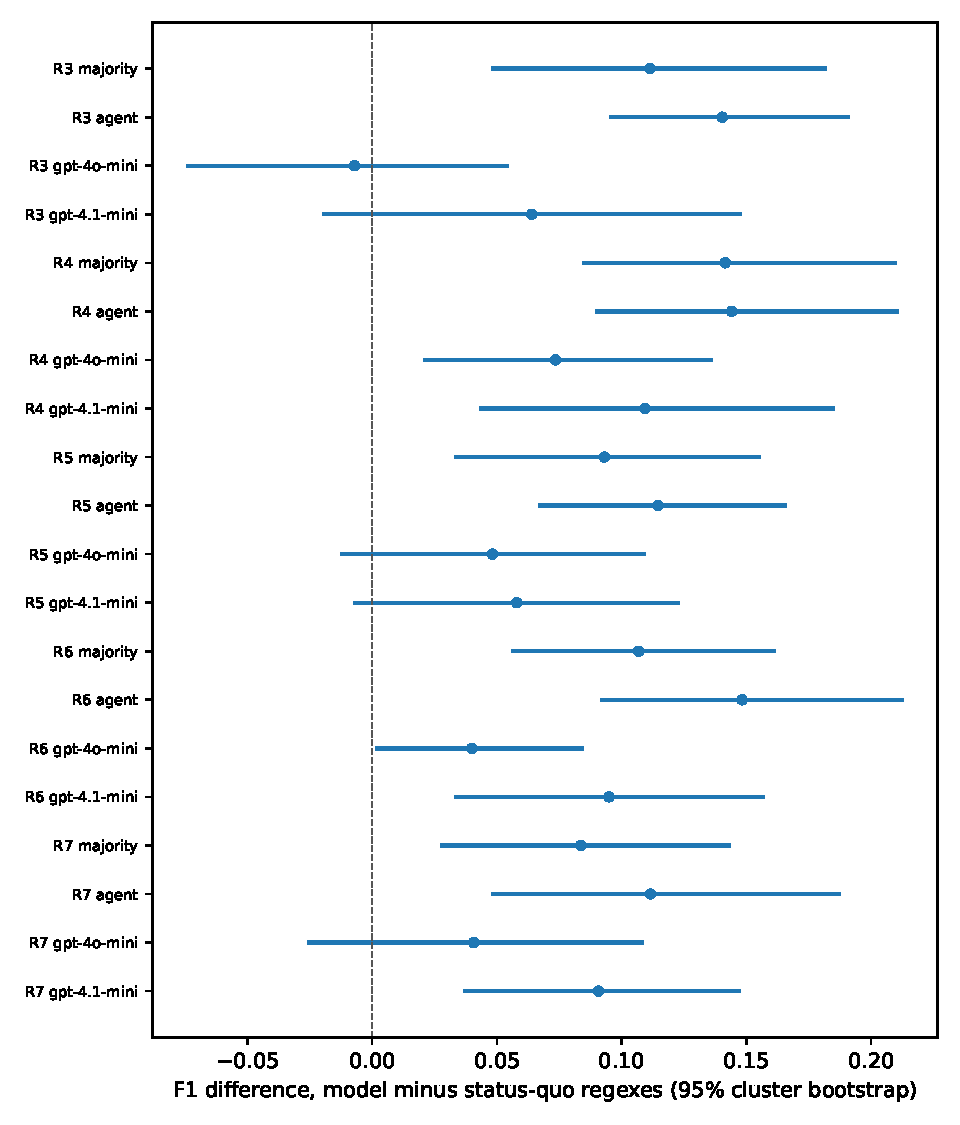
\includegraphics[width=0.75\linewidth]{fig_forest.pdf}
\caption{F1 difference (model minus status quo) per test and annotator, with 95\% cluster-bootstrap intervals.}
\end{figure}
In rounds 4, 5 and 7 every annotator's point difference is positive; in round 6 every interval is above zero; in round 3 the judge intervals include zero. H2 (specificity $\ge$ 0.70 with recall $\ge$ 0.90) holds in rounds 4--7, with thin margins in round 7 (0.703, 0.903). Gains concentrate in checklist-heavy documents (large stratum, round 4: +0.33 F1) and are small in short documents without checklists (+0.03).
\paragraph{Ceiling.} Annotators agree with each other on 75--82\% of binding-set items ($\kappa$ 0.47--0.56, Table~\ref{tab:ceiling}). The model agrees with the agent on 95\% ($\kappa$ 0.88; the agent also wrote the rules), with gpt-4o-mini on 80\% and with gpt-4.1-mini on 73\%. On items where two annotators agree, the left-out annotator matches their consensus in 81--89\% of cases, versus 87--96\% for the model depending on whose consensus is used (the model's number is inflated where the agent trained it). A score of 0.98 on all criteria is therefore not attainable against these labels without fitting to annotator-specific conventions.
\begin{table}[h]\centering\small
\begin{tabular}{lrrr}
\toprule
Pair & Items & Agreement & Cohen $\kappa$ \\
\midrule
agent vs gpt-4o-mini & 1958 & 0.821 & 0.56 \\
agent vs gpt-4.1-mini & 1807 & 0.760 & 0.49 \\
gpt-4o-mini vs gpt-4.1-mini & 1799 & 0.752 & 0.47 \\
\midrule
model vs agent & 2018 & 0.950 & 0.88 \\
model vs gpt-4o-mini & 1981 & 0.805 & 0.51 \\
model vs gpt-4.1-mini & 1821 & 0.730 & 0.43 \\
\bottomrule
\end{tabular}

\caption{Pairwise agreement on binding-set labels pooled over rounds 3 to 6.}\label{tab:ceiling}
\end{table}
\paragraph{Negative results.} (a) Retraining on 2{,}404 weak labels where two OpenAI voters agreed scored below the rule-only version on development data in all three variants. (b) A number-level stacker (logistic regression over mention probabilities, trained on the agent's labels of rounds 2 to 4) had cross-validated AUC 0.982 against 0.949 for max-q but gave $+0.004$ [$-0.003$, +0.014] F1 on a fresh round, so max-q remains the default. (c) A calibrated review queue (probability in (0.1, 0.9)) caught 58\%, 48\%, 64\% and 53\% of the errors in four rounds (targets were 60\%).
\paragraph{Remaining errors.} Construction specifications that cite clauses in running text (clean errors of rounds 4--7 are dominated by a few specification documents), clause lists without markers, documents whose checkbox markers were lost in extraction (labelled UNDECIDED), and exclusion wordings placed mid-line after the clause title (found while labelling round 7; queued for v1.5).

\section{Limitations}
(1) No human expert labels; the judge instructions derive from the agent's conventions, so the annotators are not independent readers of the format. (2) The agent that labelled also wrote the rules; rounds 2 to 7 are not independent of rule design except through freshness of documents. (3) 24--36 documents per round (27 in round 7, drawn from a one-week posting window) with recurring federal templates; the rounds are not independent draws of the template population. (4) Numbers only; alternates, dates and ranges are not in the gold. (5) A federal-contracting API sample from 2024-10 to 2026-10; one scanned-document share ($\approx$3\%) is not processed. (6) Not legal advice; the model must not remove clauses silently.

\section{Roadmap}\label{sec:roadmap}
The decision log queues: an encoder fine-tune (ModernBERT-base span classifier over layout-marked windows, the Phase-8 design the linear model stands in for), an ``applicable'' mode for narrative requirements (the REFERENCED tier, where B0 still leads), review-queue calibration, and more document templates (SF~30 amendments, lease clauses). Reinforcement learning is not on this list: the shipped system is a classifier with a fixed label schema, and its errors are concentrated in document-structure handling that rules and supervised span classification address directly; RL would first need a reward signal that does not exist (no expert preference data) and would inherit the same annotator ceiling.

\section{Release, ethics and reproducibility}\label{sec:release}
Documents are public SAM.gov attachments. Extraction redacts personal-data patterns (contact emails and phone numbers, hardened against glued tokens; verified zero remaining in the release). The release contains derived tables and short snippets, not documents. Every number is generated from \texttt{results/*.json} by scripts in the repository; decisions are logged (D-001 to D-045). Public artefacts: model weights as a pickle-free numpy archive with a numpy-only inference script (\url{https://huggingface.co/raihan-js/fedproc-ledger-v1}, Apache-2.0), dataset and round reports (\url{https://huggingface.co/datasets/raihan-js/fedproc-ledger-bench}), research code (\url{https://github.com/raihan-js/fedproc-ledger}, Apache-2.0). No Qwen or other non-US model was used. The authors are affiliated with a company that sells proposal software; this work uses only public solicitations and the integration contract keeps customer documents in-boundary.

\begin{thebibliography}{9}
\bibitem{hendrycks2021cuad} D.~Hendrycks, C.~Burns, A.~Chen, S.~Ball. CUAD: An expert-annotated NLP dataset for legal contract review. In \emph{NeurIPS}, 2021. \url{https://arxiv.org/abs/2103.06268}
\bibitem{tuggener2020ledgar} D.~Tuggener, P.~von D{\"a}niken, T.~Peetz, M.~Cieliebak. LEDGAR: a large-scale multi-label corpus for text classification of legal provisions in contracts. In \emph{LREC}, pages 1235--1241, 2020. \url{https://aclanthology.org/2020.lrec-1.155/}
\bibitem{koreeda2021contractnli} Y.~Koreeda, C.~D.~Manning. ContractNLI: a dataset for document-level natural language inference for contracts. In \emph{Findings of EMNLP}, pages 1907--1919, 2021. \url{https://arxiv.org/abs/2110.01799}
\bibitem{chalkidis2022lexglue} I.~Chalkidis et al. LexGLUE: a benchmark dataset for legal language understanding in English. In \emph{ACL}, pages 4310--4330, 2022. \url{https://aclanthology.org/2022.acl-long.297/}
\bibitem{jaume2019funsd} G.~Jaume, H.~K.~Ekenel, J.-P.~Thiran. FUNSD: a dataset for form understanding in noisy scanned documents. In \emph{ICDARW}, volume 2, pages 1--6, 2019. \url{https://arxiv.org/abs/1905.13538}
\bibitem{warner2024modernbert} B.~Warner et al. Smarter, better, faster, longer: a modern bidirectional encoder for fast, memory efficient, and long context finetuning and inference. \emph{arXiv:2412.13663}, 2024. \url{https://arxiv.org/abs/2412.13663}
\bibitem{nosek2018preregistration} B.~A.~Nosek et al. The preregistration revolution. \emph{PNAS}, 115(11):2600--2606, 2018.
\bibitem{mitchell2019modelcards} M.~Mitchell et al. Model cards for model reporting. In \emph{FAT*}, 2019.
\bibitem{gebru2021datasheets} T.~Gebru et al. Datasheets for datasets. \emph{CACM}, 64(12):86--92, 2021.
\bibitem{guo2017calibration} C.~Guo et al. On calibration of modern neural networks. In \emph{ICML}, 2017.
\bibitem{efron1993bootstrap} B.~Efron, R.~J.~Tibshirani. \emph{An Introduction to the Bootstrap}. Chapman \& Hall, 1993.
\bibitem{cohen1960} J.~Cohen. A coefficient of agreement for nominal scales. \emph{Educ.\ Psych.\ Meas.}, 20(1):37--46, 1960.
\bibitem{ecfr2026} Office of the Federal Register. Electronic Code of Federal Regulations. \url{https://www.ecfr.gov}
\end{thebibliography}
\end{document}
